% Preamble
\documentclass[11pt,pdf, aspectratio=169]{beamer}
\usetheme{metropolis}
\title{DAPC 2023 Training Sessions\\Session 3}
\author{Verwoerd}

% Packages
\usepackage{amsmath}
\usepackage[utf8]{inputenc}
\usepackage[T1]{fontenc}
\usepackage{graphicx}
\usepackage{tikz}
\usepackage{minted}
\usepackage[
  type={CC},
  modifier={by-sa},
  version={4.0},
]{doclicense}
\setsansfont{Fira Sans}
\usemintedstyle{manni}
\setminted{
  fontsize=\footnotesize,linenos,frame=lines, framesep=2mm
}

\begin{document}
  \maketitle
  \begin{frame}{Session 3}
    \begin{itemize}
      \item Team Reference Document
      \item Solutions to Sorting and Search Problems
      \item Solving interactive problems
      \item Solving Dynamic Programming Problems
    \end{itemize}
    \doclicenseThis
  \end{frame}


  \section{Team Reference Document}
  \begin{frame}{Team Reference Document}
    \begin{itemize}
      \item During the DAPC you may bring all analogue reference material you want
      \item Starting from the BAPC the World finals rules you may only bring limited amount of references
      \item This reference is called the Team Reference Document (TRD)
      \item Sometimes the old term Team Contest Reference (TCR) is used
    \end{itemize}
  \end{frame}
  \begin{frame}{Team Reference Document: Rules}
    \begin{quote}
      Each contestant may bring an \textit{(identical)} copy of a Team Reference Document.
      This document may contain up to 25 pages of reference materials, single-sided, letter or A4 size, with pages numbered in the upper right-hand corner and your university name printed in the upper left-hand corner.
      Text and illustrations must be readable by a person with correctable eyesight without magnification from a distance of ½ meter.
      It may include handwritten comments and corrections on the fronts of pages only.
      The document should be in some type of notebook or folder with the name of your institution on the front.
    \end{quote}
  \end{frame}
  \begin{frame}{TRD: Example}
    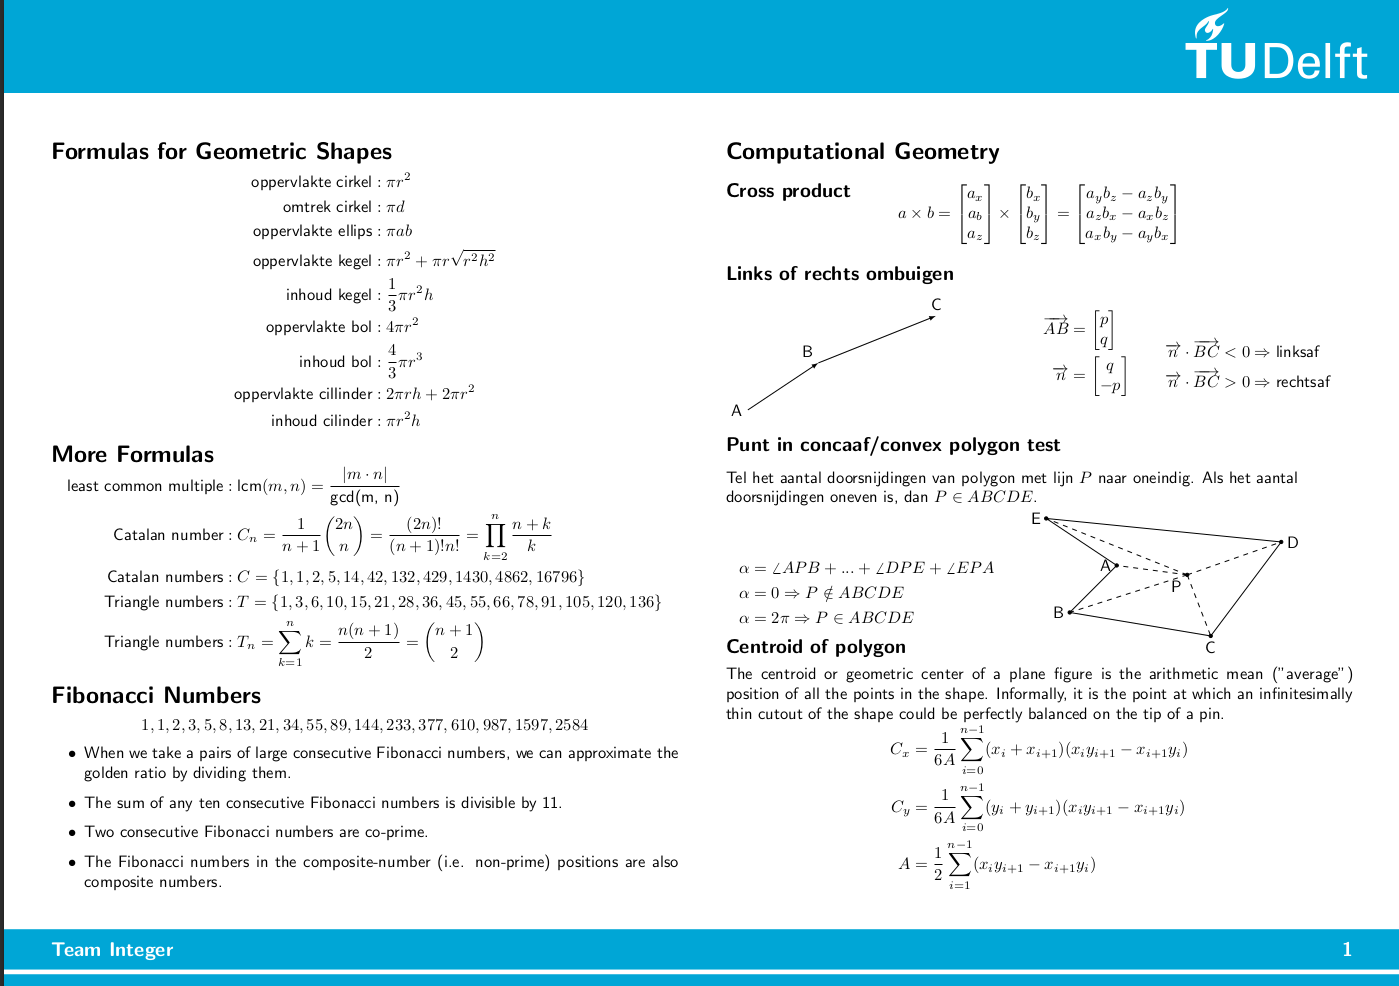
\includegraphics[width=.8\linewidth]{images/session-3/tcr-1}
  \end{frame}
  \begin{frame}{TRD: Example}
    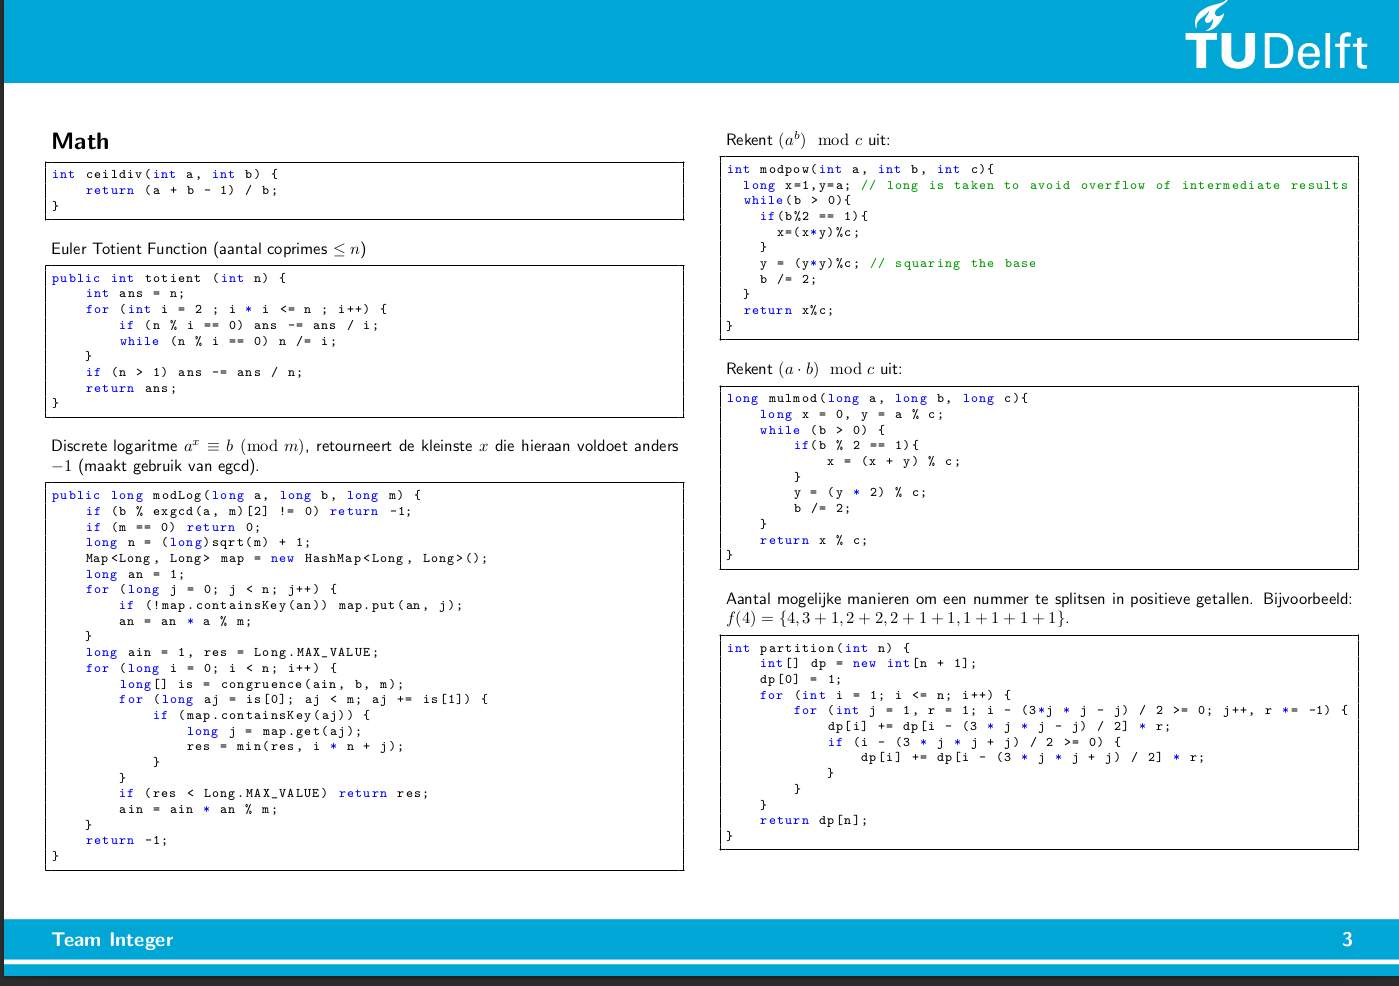
\includegraphics[width=.8\linewidth]{images/session-3/tcr-2}
  \end{frame}
  \begin{frame}{TRD: Example}
    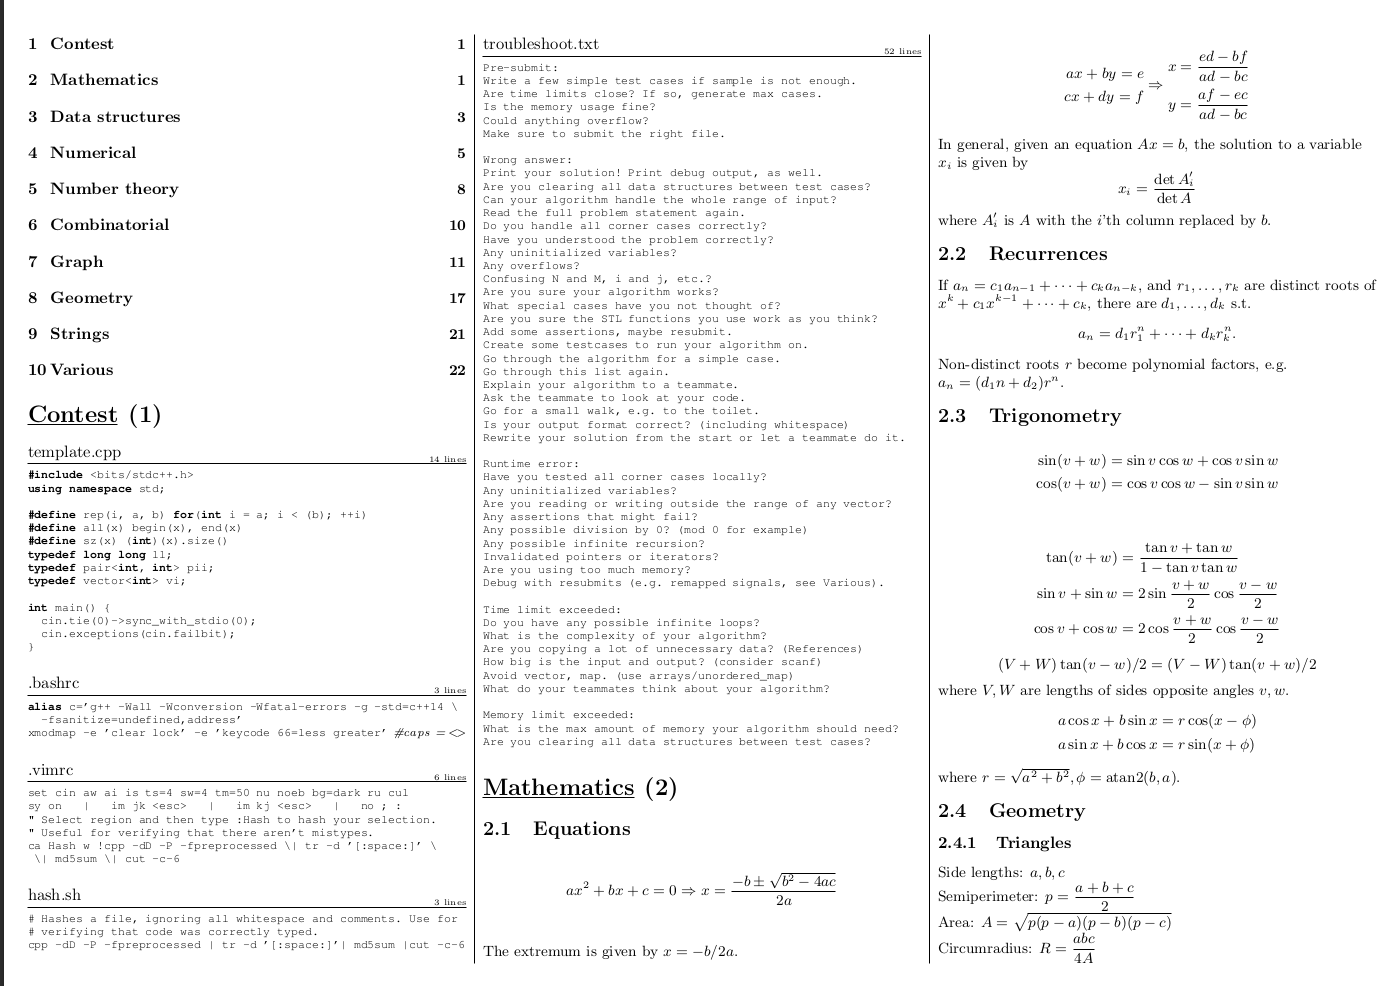
\includegraphics[width=.8\linewidth]{images/session-3/tcr-3}
  \end{frame}
  \begin{frame}{TRD: Example}
    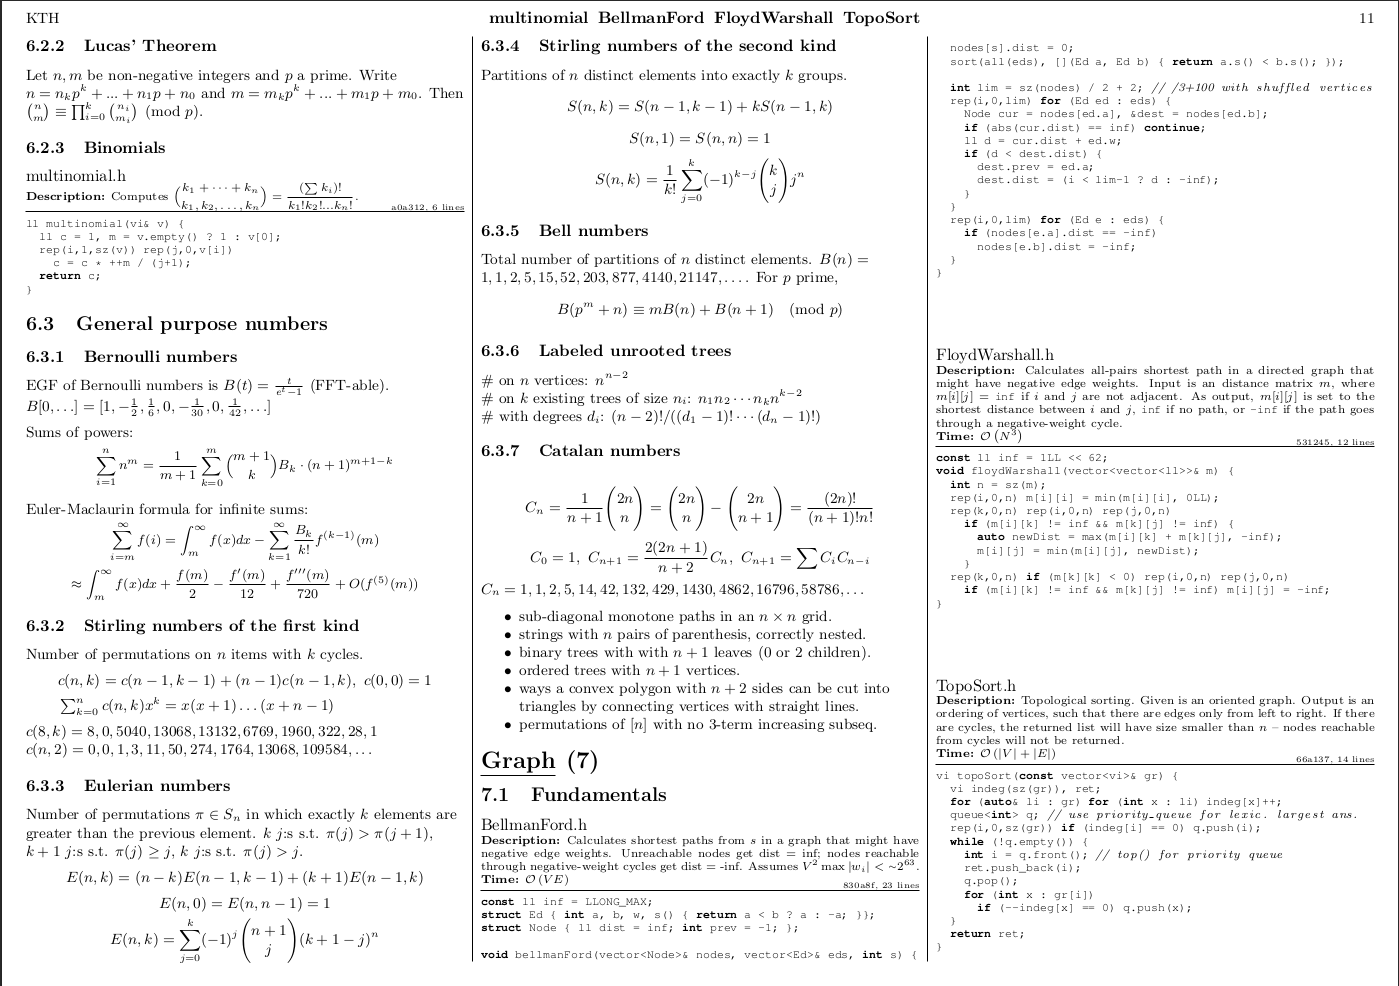
\includegraphics[width=.8\linewidth]{images/session-3/tcr-4}
  \end{frame}
  \begin{frame}{Potential subjects in a TRD}
    \begin{columns}
      \begin{column}{.45\textwidth}
        \begin{enumerate}
          \item Mathematics
          \begin{itemize}
            \item formulas and theories
            \item trigonometry
          \end{itemize}
          \item Data Structures
          \begin{itemize}
            \item Segement Tree, Treap, RMQ
            \item HashMap, PriorityQueue
          \end{itemize}
          \item Numerical Methods
          \begin{itemize}
            \item Simplex, Integration
            \item Linear Problem-solving
          \end{itemize}
          \item Number Theory
          \begin{itemize}
            \item Primality, Divisability
          \end{itemize}
          \item Combinatorial
          \begin{itemize}
            \item Permutations, Partitions
          \end{itemize}
        \end{enumerate}
      \end{column}
      \begin{column}{.45\textwidth}
        \begin{enumerate}
          \addtocounter{enumi}{5}
          \item Graph
          \begin{itemize}
            \item Search algorithms
            \item Flow algorithms
            \item Spanning Tree, Connected Components
          \end{itemize}
          \item Geometry
          \begin{itemize}
            \item Line intersection, length
            \item Triangles and Circles
            \item Polygons
          \end{itemize}
          \item Strings
          \item Templates
          \item Tests and reminders
        \end{enumerate}
      \end{column}
    \end{columns}
  \end{frame}
  \begin{frame}{Tips on TRD}
    \begin{itemize}
      \item Only put stuff in you know when to use
      \item Ensure that the code is correct and complete
      \item Add short description, complexity and hash
      \item Evaluate document after each contest for improvements
      \item Several templates available at \texttt{https://chipcie.wisv.ch/resources}
    \end{itemize}
  \end{frame}


  \section{Solutions to the sorting and search problems}
  \begin{frame}{Abbreviated Aliases}
    \begin{itemize}
      \item Source BAPC Preliminaries 2022
      \item Time limit: 2s
      \item For every username calculate the size of the shortest unique prefix.
    \end{itemize}
    Original problem written by the BAPC 2022 jury and licensed under \doclicenseLongNameRef.

    \doclicenseImage
  \end{frame}

  \begin{frame}{Abbreviated Aliases}
    \begin{itemize}
      \item Observation: The input is $10^7$, so we are aiming for a $\mathcal{O}(n\log{}n)$
      \item Comparing every username with all other usernames is $\mathcal{O}(n^2)$, which is too slow
      \item We only need to compare the two usernames where the prefix is most similar\\
      \texttt{james} is closest to \texttt{jacob} and \texttt{janos}, there is no other username that will increase the prefix
      \item If we sort the list, we only have to compare with the username before and after
      \item Alternatively, build a compressed Trie and for each leaf count the distance to the root
    \end{itemize}
  \end{frame}
  \begin{frame}[containsverbatim]{Abbreviated Aliases}
    \inputminted{python}{code/session-1/python/dapc-a.py}
  \end{frame}

  \begin{frame}{Dimensional Debugging}
    \begin{itemize}
      \item Source BAPC Preliminaries 2022
      \item Time limit: 2s
      \item Given $n$ algorithms that only work when their input $\varphi$ is small enough ($\varphi \leq H$), can you verify the correctness on sufficient large inputs($\varphi \geq L$).
    \end{itemize}
    Original problem written by the BAPC 2022 jury and licensed under \doclicenseLongNameRef.

    \doclicenseImage
  \end{frame}

  \begin{frame}{Dimensional Debugging}
    \begin{itemize}
      \item Observation: The input is $~10^4$, so we are aiming for an $\mathcal{O}(n^2)$ algorithm.
      \item We can verify all algorithms with $L = \varphi_0$
      \item Add those algorithms to verified algorithms, then find any unverified where $H_j \leq L_i$
      \item In this way you can create a graph between the different algorithms.
      \item Use a flood fill by BFS/DFS to count the number of algorithms you can reach.
      \item This results in an $\mathcal{O}(n^2)$ algorithm.
    \end{itemize}
  \end{frame}
  \begin{frame}[containsverbatim]{Dimensional Debugging}
    \inputminted[fontsize=\tiny]{python}{code/session-1/python/dapc-d.py}
  \end{frame}

  \begin{frame}{Extended Braille}
    \begin{itemize}
      \item Source BAPC Preliminaries 2022
      \item Time limit: 8s
      \item Given $n$ braille characters by their points, determine how many of them are distinct up to translation.
    \end{itemize}
    Original problem written by the BAPC 2022 jury and licensed under \doclicenseLongNameRef.

    \doclicenseImage

  \end{frame}
  \begin{frame}{Extended Braille}
    \begin{itemize}
      \item Observation 1: time limit of 8s is due to high input size
      \item Observation 2: Number of inputs is $10^6$, so we are looking for a $\mathcal{O}(n\log{}n)$
      \item Per Braille character sort the dots on $x$ then $y$
      \item Move the first ordered dot to $(0, 0)$ by subtracting the first point coordinate from all the dots\\
      $\forall^{i=0}_m (x'_i, y'_i) = (x_i - x_o, y_i - y_0)$
      \item Add the transposed characters to a Hashmap and count the unique keys
      \item Resulting a $\mathcal{O}(n\log{}n)$ or amortized $\mathcal{O}(n)$
    \end{itemize}
  \end{frame}
  \begin{frame}[containsverbatim]{Abbreviated Aliases}
    \inputminted{python}{code/session-1/python/dapc-e.py}
  \end{frame}
  \begin{frame}{Knitting Pattern}
    \begin{itemize}
      \item Source BAPC Preliminaries 2022
      \item Time limit: 3s
      \item Given a knitting pattern and amount of wool it costs for letting the wool strand unused, using the wool in a stitch, and for starting or ending the use of wool.
      Compute the minimal amount of wool required for every colour of wool.
    \end{itemize}
    Original problem written by the BAPC 2022 jury and licensed under \doclicenseLongNameRef.

    \doclicenseImage
  \end{frame}
  \begin{frame}{Knitting Pattern}
    \begin{itemize}
      \item Observation: The input is $10^6$, so we are aiming for a $\mathcal{O}(n\log{}n)$
      \item For gap between colours you have 2 options
      \begin{enumerate}
        \item let the strand continue
        \item stop the strand and start again
      \end{enumerate}
      \item For every colour we have to calculate for every gap \[\min(c_{stop}+c_{start}, gap_{size}\cdot c_{unused})\]
      \item Calculate the total cost for each colour and sum it together
      \item The complexity is $\mathcal{O}(w\cdot n)$ or can in single pass with creative bookkeeping
    \end{itemize}
  \end{frame}
  \begin{frame}[containsverbatim]{Knitting Pattern}
    \inputminted{python}{code/session-1/python/dapc-k.py}
  \end{frame}

  \begin{frame}{Kiosk Construction}
    \begin{itemize}
      \item Source BAPC 2022
      \item Time limit: 8s
      \item Find the optimal kiosk position for a given camping layout.
    \end{itemize}
    Original problem written by the BAPC 2022 jury and licensed under \doclicenseLongNameRef.

    \doclicenseImage
  \end{frame}
  \begin{frame}{Kiosk Construction}
    \begin{itemize}
      \item The shortest path for every kiosk position to every other plot can be found by using DFS/BFS
      \item Then find the kiosk(s) that can reach all plot and minimize the maximum distance
      \item Doing $n^2$ DFS/BFS for every kiosk results in a $\mathcal{O}(n^3)$ solution and receives a TLE
      \item You an optimize do to some preprocessing, calculate the distance from every plot to every kiosk position, storing intermediate results
      \item This optimization results in a $\mathcal{O}(n^2)$ solution
    \end{itemize}
  \end{frame}
  \begin{frame}[containsverbatim]{Kiosk Construction}
    \inputminted[fontsize=\tiny]{python}{code/session-1/python/bapc-k.py}
  \end{frame}


  \section{Solving interactive problems}
  \begin{frame}{What are Interactive Problems?}
    \begin{itemize}
      \item Traditional problems give all the input at once, you solve and print all the output at once
      \item Interactive problems give in put, you do work and output and you receive new input
      \item continue this process until you find the final answer
      \item The problem defines an interaction protocol
      \item The problem has an additional interaction limit
      \item Usually if an interactive problem is in the set, an simple interactive problem will be included in the test session
    \end{itemize}
  \end{frame}
  \begin{frame}{Type of probelms for Interactive Problems}
    \begin{itemize}
      \item Search in a finite space
      \item Explore a maze
      \item matching games
      \item Double interaction problem (very, very rare)
      \begin{itemize}
        \item Program has 2 modes
        \item the first mode, input transforms input to output following certain rules
        \item The second mode, the output of mode 1 is given and you have tranform it back to the input of mode 1
      \end{itemize}
    \end{itemize}
  \end{frame}
  \begin{frame}{Common pitfalls for Interactive problems}
    \begin{itemize}
      \item Flush the output after every write
      \begin{itemize}
        \item Only the output, not the input
        \item Not flushing the output results in Time Limit Exceeded
      \end{itemize}
      \item Results of the problem is not deterministic, but the following is guaranteed:
      \begin{itemize}
        \item Wrong Answer means your printed something wrong
        \item Runtime Error means you returned an 0 error code
        \item If both occur, you will get either
      \end{itemize}
    \end{itemize}
  \end{frame}
  \begin{frame}{Interactive problems testing tool}
    \begin{itemize}
      \item Most contests provide a testing tool to test the interaction with a testing tool
      \item This is usually called \texttt{testing\_tool.py} in our region
      \item The header file tells you how to run run the testing tool, for example\\\texttt{\textdollar python3 testing\_tool.py -f 1.in python3 ./solution.py}
      \item Pitfall for Java/Kotlin: You should run the testing tool in the directory which contains the compiled class file

      \item \textbf{Wrong}:\\\texttt{\textasciitilde/\textdollar python3 testing\_tool.py -f 1.in java ./code/ProblemA}
      \item \textbf{Right}:\\\texttt{\textasciitilde/code/\textdollar python3 testing\_tool.py -f 1.in java ProblemA}
    \end{itemize}
  \end{frame}
  \begin{frame}{example interactive problem}
    You are asked to guess a number between 0 and $n$.
  \end{frame}
  \begin{frame}{example interactive problem: Interaction}
    This is an interactive problem.
    Your submission will be run against an interactor, which reads from the standard output of your submission and writes to the standard input of your submission.
    This interaction needs to follow a specific protocol:

    The interactor first sends one line with an integer $n$ ( $3 \leq n \leq 1000$), the upper bound of the guessing game.

    You can then send a guess $g$ ($0\leq g \leq n$).

    The interactor will respond with the strings \texttt{lower}, \texttt{higher} or \texttt{correct}.
    This represents is if the number to guess is lower, higher or correct respectivly.
    After you have guessed the correct number, you should exit the program.

    The interactor is not adaptive, i.e., the secret number is fixed during a round.
    Using more than 12 guesses will result in a wrong answer.
  \end{frame}
\end{document}
